\section{Máy biến áp - Truyền tải điện năng}
\subsection{Tóm tắt lí thuyết}
\begin{tomtat}
	\subsubsection{Máy biến áp}
	\begin{dn}
		Máy biến áp là thiết bị biến đổi điện áp của dòng điện xoay chiều \textit{(nhưng không làm thay đổi tần số của dòng điện xoay chiều)}.
	\end{dn}
	\paragraph{Cấu tạo và nguyên tắc hoạt động}
	\begin{enumerate}[label=\bfseries \alph*)]
		\item \textbf{Cấu tạo}\\
			\begin{tabular}{L{10cm}M{6cm}}
				\begin{itemize}
					\item Một lõi thép hình khung chữ nhật gồm  nhiều lá thép mỏng ghép cách điện với nhau.
					\begin{luuy}
						Phải dùng các lá sắt hoặc thép pha silicon ghép cách điện với nhau để giảm hao phí điện năng do dòng điện Foucault.\end{luuy}
					\item Hai cuộn dây đồng có số vòng dây khác nhau quấn trên lõi thép. Một cuộn nối với mang điện xoay chiều gọi là \textit{\textbf{cuộn sơ cấp}}. Cuộn kia nối với tải tiêu thụ điện gọi là \textit{\textbf{cuộn thứ cấp}}.
				\end{itemize}& 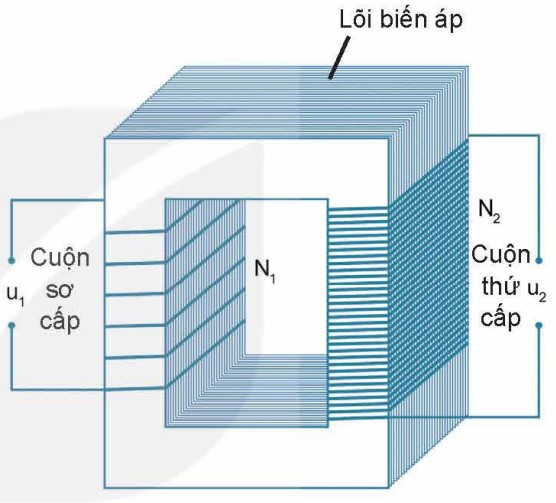
\includegraphics[width=0.8\linewidth]{figs/VN12-Y24-PH-SYL-024-1}
				\captionof{figure}{Cấu tạo đơn giản của máy biến áp.}\\
			\end{tabular}
		\item \textbf{Nguyên tắc hoạt động}\\
		Máy biến áp hoạt động dựa trên \textbf{\textit{hiện tượng cảm ứng điện từ}}.\\
		Dòng điện xoay chiều chạy trong cuộn sơ cấp gây ra từ thông biến thiên qua cuộn thứ cấp, làm xuất hiện trong cuộn thứ cấp một suất điện động xoay chiều thay đổi theo thời gian. Khi đó, nếu đo điện áp xoay chiều $u_2$ ở hai đầu cuộn thứ cấp thì thu được giá trị của nó thay đổi theo thời gian tương ứng. Nếu mạch thứ cấp kín thì có dòng điện chạy trong cuộn thứ cấp.
	\end{enumerate}
	\paragraph{Sự biến đổi điện áp và cường độ dòng điện}
	\begin{enumerate}[label=\bfseries \alph*)]
		\item \textbf{Sự biến đổi điện áp}\\
		\begin{boxdl}
			Tỉ số điện áp ở hai đầu cuộn thứ cấp và cuộn sơ cấp bằng tỉ số vòng dây hai cuộn:
			\begin{equation}
				\dfrac{U_2}{U_1}=\dfrac{N_2}{N_1}
			\end{equation}
		\end{boxdl}
		trong đó
		\begin{itemize}
			\item $U_1$; $U_2$: điện áp hiệu dụng hai đầu cuộn sơ cấp và thứ cấp, đơn vị trong hệ SI là volt $\left(\si{\volt}\right)$;
			\item $N_1$; $N_2$: số vòng dây cuộn sơ cấp và thứ cấp.
		\end{itemize}
		\item \textbf{Sự biến đổi cường độ dòng điện}\\
	\begin{boxdl}
		Nếu bỏ qua hao phí năng lượng trong máy biến áp thì:
		$$\calP_1=\calP_2\Leftrightarrow U_1I_1=U_2I_2.$$
	\end{boxdl}
		Như vậy:
		\begin{equation}
			\dfrac{U_2}{U_1}=\dfrac{I_1}{I_2}
		\end{equation}
		với $I_1$; $I_2$ là cường độ dòng điện hiệu dụng qua cuộn sơ cấp và thứ cấp.
	\end{enumerate}
	\paragraph{Ứng dụng của máy biến áp}
	\begin{itemize}
		\item Biến đổi điện áp phù hợp với nhu cầu sử dụng.
		\item Tăng điện áp khi truyền tải điện năng để giảm hao phí trên đường dây tải.
		\item Hàn điện, nấu chảy kim loại, \dots trong đó cuộn sơ cấp có nhiều vòng dây tiết diện nhỏ, cuộn thứ cấp có ít vòng dây tiết diện lớn để tăng cường độ dòng điện qua tải ở cuộn thứ cấp.
	\end{itemize}
	\subsubsection{Truyền tải điện năng}
	Điện năng sản xuất từ nhà máy điện được truyền tải đến nơi tiêu thụ nhờ đường dây dẫn.\\
	\begin{itemize}
		\item Công suất tải đi trên đường dây dẫn:
		\begin{equation}
			\calP=UI\cos\varphi\Rightarrow I=\dfrac{\calP}{U\cos\varphi}
		\end{equation}
		trong đó:
		\begin{itemize}
			\item $U$: điện áp hiệu dụng ở hai đầu đường truyền, đơn vị trong hệ SI là volt $\left(\si{\volt}\right)$;
			\item $I$: cường độ dòng điện hiệu dụng trên dây, đơn vị trong hệ SI là ampere $\left(\si{\ampere}\right)$;
			\item $\cos\varphi$: hệ số công suất của đường dây truyền tải điện.
		\end{itemize}
		\item Dây dẫn điện có điện trở $r$, do đó công suất hao phí do toả nhiệt trên đường dây là
		\begin{equation}
			\Delta \calP=I^2r=\dfrac{\calP^2r}{U^2\cos^2\varphi}
		\end{equation}
	\begin{noidung}{}
		Với $\calP$ xác định, muốn giảm $\Delta \calP$ thì:
		\begin{itemize}
			\item giảm $r$ bằng cách tăng tiết diện dây dẫn. Cách này không khả thi vì tốn kém.
			\item tăng $U$ bằng cách dùng máy biến áp tăng điện áp ở nơi phát, ở nơi thu dùng máy biến áp để giảm điện áp. Cách này được sử dụng chủ yếu hiện nay. 
		\end{itemize}
	\end{noidung}
		\item Độ giảm điện áp (độ giảm thế) trên đường dây
		\begin{equation}
			\Delta U=Ir
		\end{equation}
	\end{itemize}
\end{tomtat}
\subsection{Ví dụ minh hoạ}
\begin{dang}{Vận dụng được hệ thức liên hệ giữa điện áp và số vòng dây quấn trên hai cuộn dây}
	\end{dang}
\begin{vd}
	Một máy biến áp dùng làm máy giảm áp gồm cuộn dây 100 vòng và cuộn dây 500 vòng. Bỏ qua mọi hao phí trên máy biến áp. Khi nối hai đầu cuộn sơ cấp với điện áp $u=\xsi{100\sqrt{2}\cos100\pi t}{\volt}$ thì điện áp hiệu dụng ở hai đầu cuộn thứ cấp bằng bao nhiêu?
	\loigiai{Vì là máy giảm áp nên $N_2<N_1\Rightarrow N_1=500; N_2=100$.\\
		Điện áp hiệu dụng hai đầu cuộn sơ cấp: $U_1=\dfrac{U_0}{\sqrt{2}}=\SI{100}{\volt}$.\\
		Điện áp hiệu dụng hai đầu cuộn thứ cấp:
		$$\dfrac{U_2}{U_1}=\dfrac{N_2}{N_1}\Rightarrow U_2=U_1\dfrac{N_2}{N_1}=\left(\SI{100}{\volt}\right)\cdot\dfrac{100}{500}=\SI{20}{\volt}.$$}
\end{vd}
% ========================================
\begin{vd}
Một máy biến áp có cuộn sơ cấp 1000 vòng dây được mắc vào mạng điện xoay chiều có điện áp hiệu dụng $\SI{220}{\volt}$. Khi đó, điện áp hiệu dụng ở hai đầu cuộn thứ cấp để hở là $\SI{484}{\volt}$. Bỏ qua mọi hao phí trên máy biến áp. Xác định số vòng dây quấn trên cuộn thứ cấp.
\loigiai{
Số vòng dây quấn của cuộn thứ cấp:
$$\dfrac{U_2}{U_1}=\dfrac{N_2}{N_1}\Rightarrow N_2=\dfrac{U_2}{U_1}N_1=\dfrac{\left(\SI{484}{\volt}\right)}{\left(\SI{220}{\volt}\right)}\cdot1000=\SI{2200}{\text{vòng}}.$$
}
\end{vd}
\begin{dang}{Bài toán thay đổi số vòng dây quấn trên máy biến áp}
	\end{dang}
	\begin{vd}
		Đặt vào hai đầu cuộn sơ cấp của một máy biến áp lí tưởng (bỏ qua hao phí) một điện áp xoay chiều có giá trị hiệu dụng không đổi thì điện áp hiệu dụng giữa hai đầu cuộn thứ cấp để hở là $\SI{100}{\volt}$. Ở cuộn thứ cấp, nếu giảm bớt $n$ vòng dây thì điện áp hiệu dụng giữa hai đầu để hở của nó là $U$, nếu tăng thêm $n$ vòng dây thì điện áp đó là $2U$. Nếu tăng thêm $3n$ vòng dây ở cuộn thứ cấp thì điện áp hiệu dụng giữa hai đầu để hở của cuộn này bằng bao nhiêu?
		\loigiai{
		Ban đầu:
		$$\dfrac{N_1}{N_2}=\dfrac{U_1}{U_2}=\dfrac{U_1}{100}.$$
		Sau khi lần lượt giảm $n$ vòng và tăng $n$ vòng ở cuộn thứ cấp thì:
		\begin{align*}
			\begin{cases}
				\dfrac{N_1}{N_2-n}=\dfrac{U_1}{U}\\
				\ \\
				\dfrac{N_1}{N_2+n}=\dfrac{U_1}{2U}
			\end{cases}
			\Rightarrow \dfrac{N_2+n}{N_2-n}=2\Rightarrow N_2=3n.
		\end{align*}
		Khi quấn thêm $3n$ vòng, ta có:
		$$\dfrac{U_1}{U'_2}=\dfrac{N_1}{N_2+3n}=\dfrac{N_1}{2N_2}\Rightarrow\dfrac{2U_1}{U'_2}=\dfrac{N_1}{N_2}=\dfrac{U_1}{100}\Rightarrow U'_2=\SI{200}{\volt}.$$
		}
	\end{vd}
% =======================================================
\begin{vd}
Cuộn sơ cấp của máy biến áp hạ áp có 1200 vòng, điện áp xoay chiều đặt vào cuộn sơ cấp là $\SI{100}{\volt}$. Theo tính toán thì điện áp hiệu dụng hai đầu thứ cấp để hở là $\SI{60}{\volt}$ nhưng vì có một số vòng dây của cuộn thứ cấp quấn theo chiều ngược lại so với đa số vòng còn lại nên điện áp hiệu dụng hai đầu thứ cấp chỉ là $\SI{40}{\volt}$. Bỏ qua mọi hao phí trong máy biến áp. Xác định số vòng dây bị quấn ngược.
\loigiai{
Nếu quấn đúng thì số vòng dây cuộn thứ cấp là
$$\dfrac{N_2}{N_1}=\dfrac{U_2}{U_1}\Leftrightarrow N_2=\dfrac{N_1U_2}{U_1}	=\SI{720}{\text{vòng}}.$$
Gọi $x$ là số vòng dây quấn sai. $x$ vòng dây quấn sai này gây ra từ thông ngược với $x$ vòng quấn đúng. Do đó, số vòng dây tham gia tạo ra suất điện động cảm ứng ở cuộn thứ cấp là $N_3=720-2x$.
$$\dfrac{U_1}{U_3}=\dfrac{N_1}{N_3}\Leftrightarrow \dfrac{100}{40}=\dfrac{1200}{720-2x}\Rightarrow x=\SI{120}{\text{vòng}}.$$
}
\end{vd}
\begin{dang}{Bài toán truyền tải điện năng}
\end{dang}
\begin{vd}
Ở đầu đường dây tải điện người ta truyền đi công suất điện $\SI{36}{\mega\watt}$ với điện áp $\SI{220}{\kilo\volt}$. Điện trở tổng cộng của đường dây tải điện là $\SI{20}{\ohm}$. Coi cường độ dòng điện và điện áp biến đổi cùng pha. Công suất hao phí trên đường dây tải điện có giá trị bằng bao nhiêu?
\loigiai{
Do cường độ dòng điện và điện áp biến đổi cùng pha nên $\varphi=\varphi_u-\varphi_i=\SI{0}{\radian}$.\\
Công suất hao phí trên đường dây tải điện:
$$\Delta \calP=\dfrac{\calP^2 r}{U^2\cos^2\varphi}=\dfrac{\left(\SI{36E6}{\watt}\right)^2\cdot\left(\SI{20}{\ohm}\right)}{\left(\SI{220E3}{\volt}\right)^2\cos^20}=\SI{0.54}{\mega\watt}.$$	
}
\end{vd}
% =========================================
\begin{vd}
Một đường dây có điện trở $\SI{4}{\ohm}$ dẫn một dòng điện xoay chiều một pha từ nơi sản xuất đến nơi tiêu dùng. Hiệu điện thế hiệu dụng ở nguồn lúc phát ra là $U=\SI{10}{\kilo\volt}$, công suất điện là $\SI{400}{\kilo\watt}$. Hệ số công suất của mạch điện là $\cos\varphi=0,8$. Có bao nhiêu phần trăm công suất bị mất mát trên đường dây do toả nhiệt.
\loigiai{
Công suất bị mất mát trên đường dây do toả nhiệt:
$$\Delta \calP=\dfrac{r\calP^2}{U^2\cos^2\varphi}.$$
Phần trăm công suất bị mất mát trên đường dây do toả nhiệt:
$$\dfrac{\Delta \calP}{\calP}=\dfrac{r\calP}{U^2\cos^2\varphi}=\SI{2.5}{\percent}.$$	
}
\end{vd}
% =====================================
\begin{vd}
Một nông trại dùng các bóng đèn dây tóc loại $\SI{200}{\watt}-\SI{200}{\volt}$ để thắp sáng và sưởi ấm vườn trồng thanh long vào ban đêm. Biết điện năng được truyền đến nông trại từ một trạm phát, giá trị điện áp hiệu dụng tại trạm phát này là $\SI{1000}{\volt}$, đường dây một pha tải điện đến nông trại có điện trở thuần $\SI{20}{\ohm}$ và máy hạ áp tại nông trại là máy hạ áp lí tưởng. Coi rằng hao phí điện năng chỉ xảy ra trên đường dây tải. Số bóng đèn tối đa mà nông trại có thể sử dụng để các đèn vẫn sáng bình thường là bao nhiêu?
\loigiai{
Gọi công suất tại nơi phát là $\calP$, công suất hao phí trên đường truyền là $\Delta\calP$ và số bòng đèn là $n$.\\
Ta có:
$$\calP-\Delta \calP=200n\Leftrightarrow \calP-\dfrac{r\calP^2}{U^2}=200n\Leftrightarrow 2\calP^2-10^5\calP+2\cdot10^7=0$$
Để phương trình trên có nghiệm $\calP$ thì $\Delta=10^{10}-16\cdot10^7n\ge 0\Leftrightarrow n\le 62,5.$\\
Vậy số bóng đèn tối đa có thể sử dụng là 62 bóng.
}
\end{vd}
\subsection{Bài tập}
\subsubsection{Trắc nghiệm nhiều phương án lựa chọn}
\setcounter{ex}{0}
\Opensolutionfile{ans}[ans/VN12-Y24-PH-SYL-023P-TN]
% ===================================================================
\begin{ex}
	Nhận định nào sau đây là \textbf{đúng} khi nói về dòng điện xoay chiều?
	\choice
	{Dòng điện xoay chiều được sử dụng rộng rãi nhờ được sản xuất ở các nhà máy có công suất lớn}
	{Dòng điện xoay chiều có điện áp lớn nên được sử dụng rộng rãi}
	{\True Dòng điện xoay chiều được sử dụng rộng rãi nhờ ưu thế dễ truyền tải đi xa nhờ máy biến áp}
	{Dòng điện xoay chiều được sử dụng rộng rãi nhờ có nhiều tác dụng hơn dòng điện một chiều}
	\loigiai{}
\end{ex}
% ===================================================================
\begin{ex}
	Nhận định nào sau đây là \textbf{đúng} khi nói về máy biến áp?
	\choice
	{\True Máy biến áp là thiết bị biến đổi điện áp xoay chiều nhưng không làm thay đổi tần số dòng điện}
	{Máy biến áp là thiết bị biến đổi điện áp xoay chiều cả về độ lớn và tần số của dòng điện}
	{Máy biến áp là thiết bị không tiêu thụ điện năng, chỉ chuyển hoá điện áp của dòng điện}
	{Máy biến áp là thiết bị hoạt động dựa trên hiện tượng cảm ứng điện từ có phần lõi sắt là nam châm vĩnh cửu}
	\loigiai{}
\end{ex}
% ===================================================================
\begin{ex}
	Nhận định nào sau đây là \textbf{không đúng} khi nói về vai trò của máy biến áp trong truyền tải điện năng?	
	\choice
	{\True Máy biến áp có vai trò quan trọng trong chuyển đổi dòng một chiều thành dòng xoay chiều giúp dòng điện xoay chiều được sử dụng rộng rãi hiện nay}
	{Máy biến áp có vai trò lớn trong truyền tải điện năng đi xa, giúp giảm hao phí trên đường truyền}
	{Máy biến áp có vai trò quan trọng trong truyền tải dòng điện xoay chiều giúp tăng điện áp trước khi truyền và giảm điện áp ở nơi sử dụng}
	{Máy biến áp có vai trò lớn trong việc giảm chi phí truyền tải điện năng từ nhà máy đến nơi sử dụng}
	\loigiai{}
\end{ex}
% ===================================================================
\begin{ex}
	Đối với máy biến áp lí tưởng, cuộn sơ cấp có $N_1$ vòng dây, cuộn thứ cấp có $N_2$ vòng dây. Cuộn thứ cấp nối với điện trở thành mạch kín, khi máy hoạt động, điện áp và cường độ dòng điện hiệu dụng ở cuộn sơ cấp và thứ cấp lần lượt là $U_1$, $I_1$ và $U_2$, $I_2$. Mối liên hệ nào sau đây là \textbf{sai}?	
	\choice
	{$\dfrac{N_1}{N_2}=\dfrac{I_2}{I_1}$}
	{\True $\dfrac{N_1}{N_2}=\dfrac{U_2}{U_1}$}
	{$\dfrac{U_2}{U_1}=\dfrac{I_1}{I_2}$}
	{$\dfrac{N_1}{U_1}=\dfrac{N_2}{U_2}$}
	\loigiai{}
\end{ex}
% ===================================================================
\begin{ex}
	Để giảm bớt hao phí do toả nhiệt trên đường dây khi cần tải điện năng đi xa bằng dòng điện xoay chiều, có thể dùng biện pháp
	\choice
	{\True tăng hiệu điện thế ở nơi sản xuất điện lên $n$ lần để giảm hao phí do toả nhiệt trên đường dây $n^2$ lần}
	{xây dựng nhà máy gần nơi tiêu thụ điện để giảm chiều dài đường dây truyền tải điện}
	{giảm hiệu điện thế máy phát điện $n$ lần để giảm cường độ dòng điện trên dây $n$ lần, giảm công suất toả nhiệt xuống $n^2$ lần}
	{dùng dây dẫn bằng vật liệu siêu dẫn có đường kính lớn}
	\loigiai{}
\end{ex}
% ===================================================================
\begin{ex}
	Trong cuộn thứ cấp của máy biến áp có 1000 vòng dây quấn xuất hiện suất điện động bằng $\SI{600}{\volt}$. Nếu máy biến áp được nối vào mạng điện với hiệu điện thế $\SI{120}{\volt}$ thì số vòng trong cuộn sơ cấp là
	\choice
	{500 vòng}
	{400 vòng}
	{600 vòng}
	{\True 200 vòng}
	\loigiai{
		$$\dfrac{N_1}{N_2}=\dfrac{U_1}{U_2}\Rightarrow N_1=200.$$
	}
\end{ex}
% ===================================================================
\begin{ex}
	Một máy biến áp có cuộn sơ cấp gồm 3300 vòng dây. Mắc cuộn sơ cấp vào mạng điện xoay chiều có hiệu điện thế hiệu dụng $\SI{220}{\volt}$ thì ở hai đầu cuộn thứ cấp để hở có một hiệu điện thế hiệu dụng $\SI{12}{\volt}$. Bỏ qua hao phí của máy biến áp. Số vòng dây của cuộn thứ cấp bằng
	\choice
	{360 vòng}
	{\True 180 vòng}
	{120 vòng}
	{90 vòng}
	\loigiai{
		$$\dfrac{N_2}{N_1}=\dfrac{U_2}{U_1}\Rightarrow N_2=180.$$	
	}
\end{ex}
% ===================================================================
\begin{ex}
	Lõi máy biến áp nóng lên khi hoạt động chủ yếu là do
	\choice
	{tác dụng nhiệt của dòng điện xoay chiều chạy trong cuộn dây sơ cấp}
	{tác dụng nhiệt của dòng điện xoay chiều chạy từ cuộn sơ cấp sang cuộn thứ cấp}
	{\True tác dụng nhiệt của dòng điện cảm ứng xuất hiện trong lõi thép khi có từ thông biến thiên qua lõi thép}
	{tác dụng nhiệt của dòng điện xoay chiều chạy trong cuộn thứ cấp nối với mạch ngoài}
	\loigiai{}
\end{ex}
% ===================================================================
\begin{ex}
	Máy hàn điện nấu chảy kim loại hoạt động theo nguyên tắc biến áp, trong đó số vòng dây và tiết diện dây của cuộn sơ cấp máy biến áp là $N_1$, $S_1$, của cuộn thứ cấp là $N_2$, $S_2$. So sánh nào sau đây là \textbf{đúng}?
	\choice
	{\True $N_1>N_2$, $S_1<S_2$}
	{$N_1>N_2$, $S_1>S_2$}
	{$N_1<N_2$, $S_1<S_2$}
	{$N_1<N_2$, $S_1>S_2$}
	\loigiai{
		Máy hàn điện hoạt động theo nguyên tắc máy biến áp, trong đó cuộn sơ cấp gồm nhiều vòng dây tiết diện nhỏ, cuộn thứ cấp gồm ít vòng dây tiết diện lớn.	
	}
\end{ex}
% ===================================================================
\begin{ex}
	Biến áp có cuộn sơ cấp 200 vòng, cuộn thứ cấp 10 vòng; điện áp và cường độ hiệu dụng ở mạch sơ cấp là $\SI{120}{\volt}$ và $\SI{0.5}{\ampere}$. Bỏ qua hao phí, điện áp và cường độ hiệu dụng ở cuộn thứ cấp là
	\choice
	{\True $\SI{6}{\volt}$; $\SI{10}{\ampere}$}
	{$\SI{60}{\volt}$; $\SI{5}{\ampere}$}
	{$\SI{12}{\volt}$; $\SI{6}{\ampere}$}
	{$\SI{12}{\volt}$; $\SI{3}{\ampere}$}
	\loigiai{
		$$\dfrac{U_2}{U_1}=\dfrac{N_2}{N_1}=\dfrac{I_1}{I_2}\Rightarrow U_2=\SI{6}{\volt}, I_2=\SI{10}{\ampere}.$$	
	}
\end{ex}

% ===================================================================
\begin{ex}
Hình bên trình bày một sơ đồ phân loại đồng xu trong máy bán hàng tự động. Có một máng nghiêng cho đồng xu chuyển động từ khe thả đồng xu đến nam châm điện. Nếu không có lực nào cản chuyển động của đồng xu hoặc lực cản rất nhỏ thì đồng xu sẽ đập vào khối chắn, rơi theo hướng bị loại, không được chấp nhận để mua hàng.
\begin{center}
	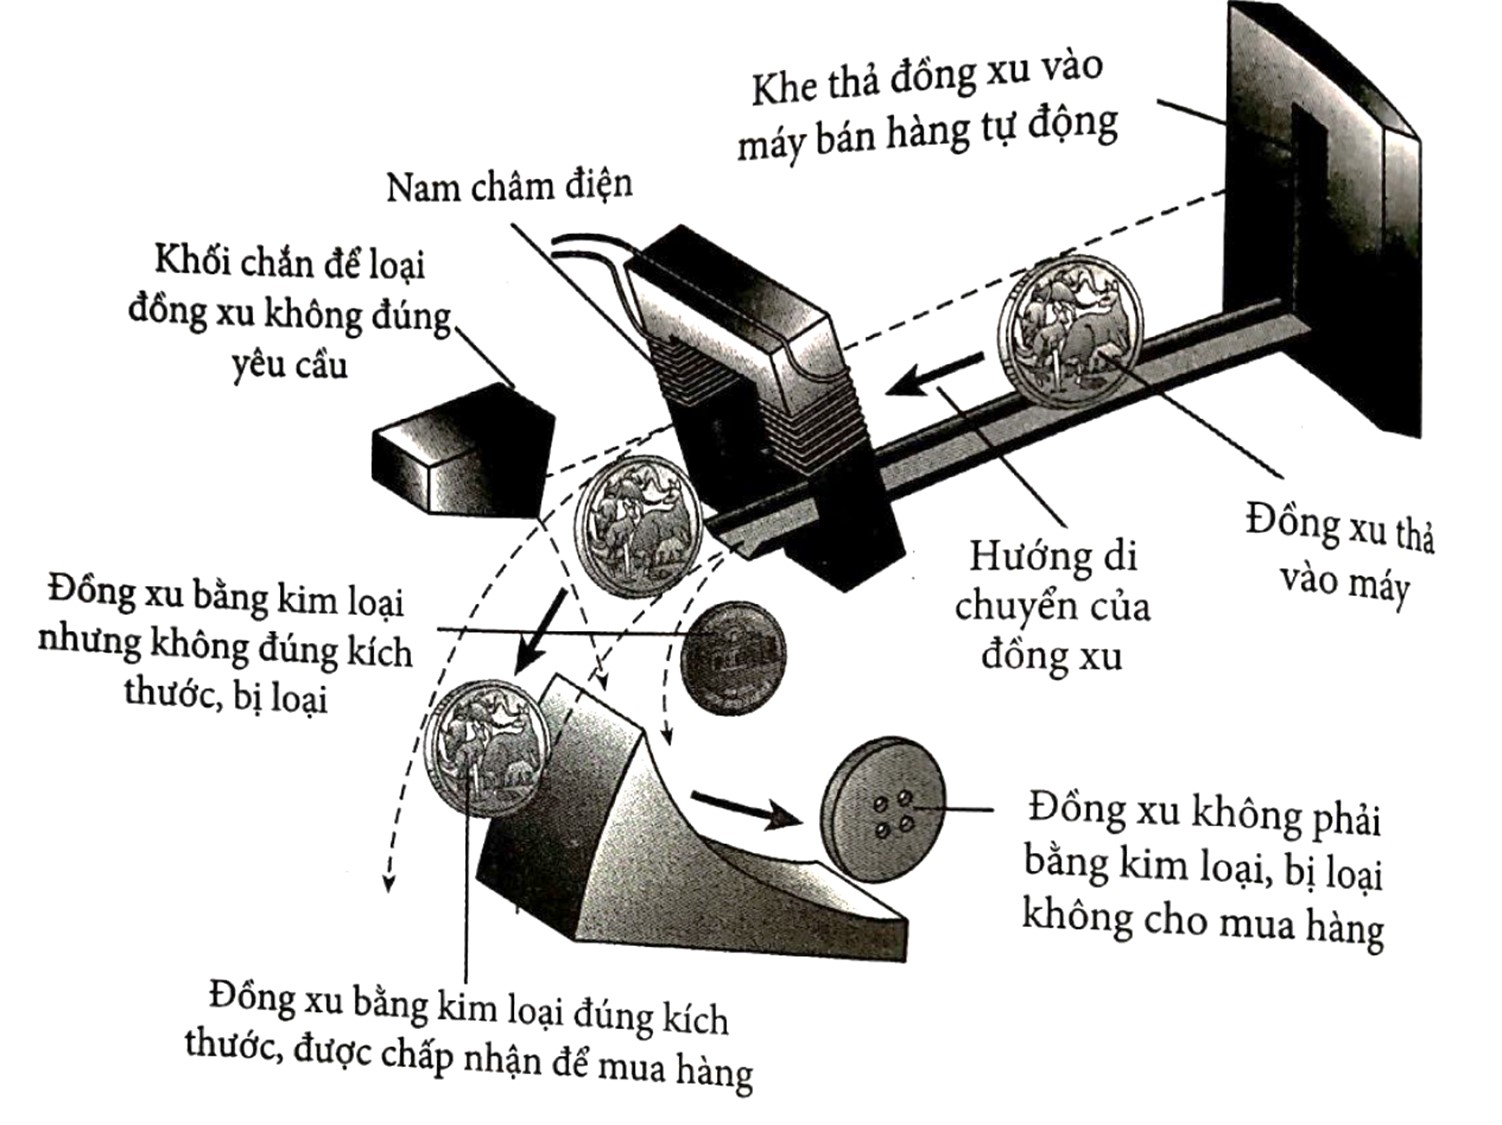
\includegraphics[scale=0.35]{figs/VN12-Y24-PH-SYL-024P-1}
\end{center}
		Phát biểu nào sau đây là \textbf{đúng}?

	\choice
	{\True Đồng xu làm bằng kim loại khi đi qua nam châm điện sẽ có hiện tượng cảm ứng điện từ, sinh ra dòng cảm điện cảm ứng trong đồng xu}
	{Chỉ cần đồng xu làm bằng kim loại với kích thước bất kì đều được chấp nhận để mua hàng}
	{Đồng xu làm bằng nhựa có khối lượng bằng đồng xu kim loại khi qua nam châm điện đều có tốc độ như nhau}
	{Không có dòng điện Foucault xuất hiện trong đồng xu kim loại khi đi qua nam châm điện}
	\loigiai{}
\end{ex}
% ===================================================================
\begin{ex}
	Khi truyền tải điện năng bằng điện áp $\SI{6}{\kilo\volt}$ thì hao phí điện năng là $\SI{50}{\percent}$. Nếu tăng điện áp truyền tải lên $\SI{12}{\kilo\volt}$ thì hao phí điện năng sẽ là
	\choice
	{$\SI{25}{\percent}$}
	{\True $\SI{12.5}{\percent}$}
	{$\SI{6.25}{\percent}$}
	{$\SI{10}{\percent}$}
	\loigiai{
		$$\calP_{\text{hp}}=\dfrac{\calP^2r}{U^2\cos^2\varphi}\Rightarrow\dfrac{\calP'_{\text{hp}}}{\calP_{\text{hp}}}=\left(\dfrac{U}{U'}\right)^2=\dfrac{1}{4}.$$
	}
\end{ex}
\Closesolutionfile{ans}
\subsubsection{Trắc nghiệm đúng/sai}
\setcounter{ex}{0}
\Opensolutionfile{ans}[ans/VN12-Y24-PH-SYL-023P-TF]
% ===================================================================
\begin{ex}
Sạc không dây hoạt động dựa trên hiện tượng cảm ứng điện từ như máy biến áp. Kết nối được thực hiện giữa hai cuộn cảm: dòng điện xoay chiều qua cuộn sơ cấp biến thiên sẽ sinh ra suất điện động cảm ứng trong cuộn thứ cấp để sạc pin điện thoại.
\begin{center}
	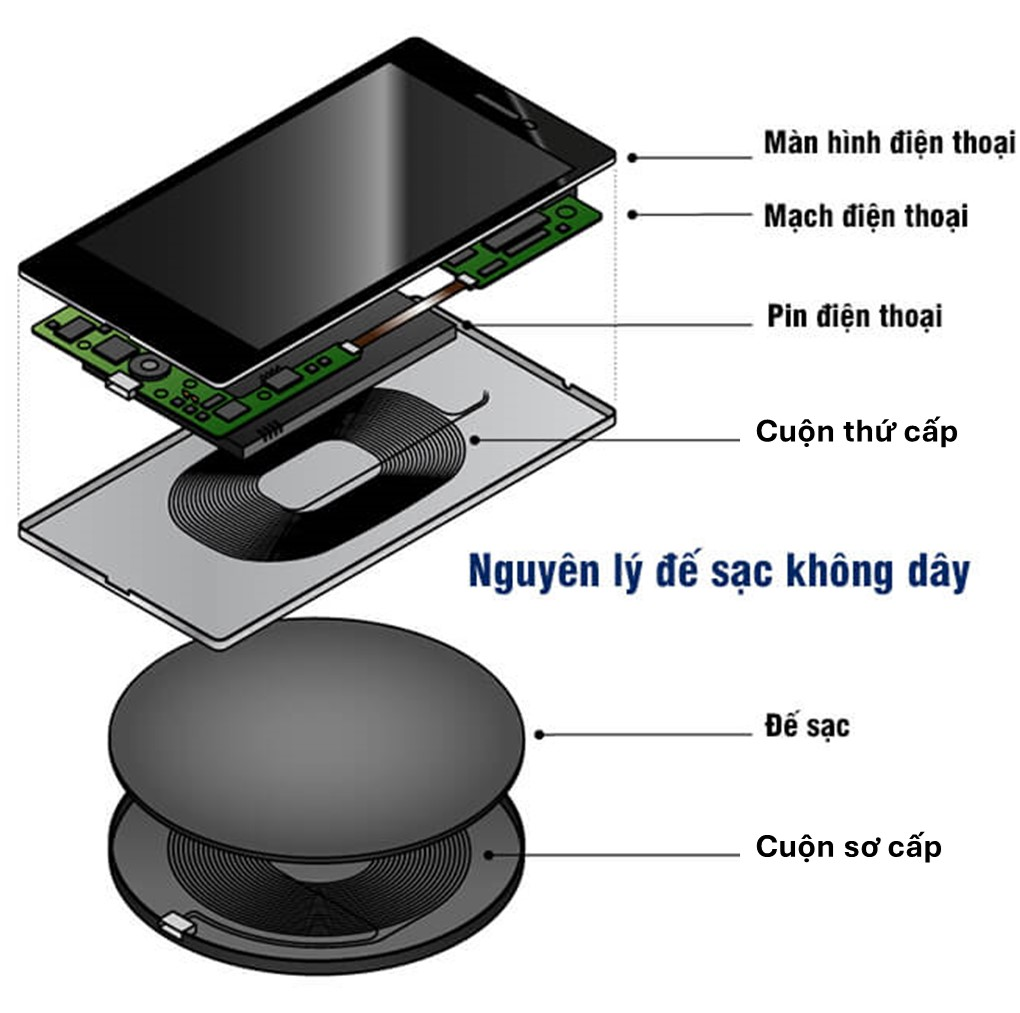
\includegraphics[scale=0.4]{figs/VN12-Y24-PH-SYL-024P-3}
\end{center}
	\choiceTF[t]
	{\True Cuộn dây trong sạc không dây (cuộn sơ cấp) được nối với dòng điện xoay chiều để tạo ra từ trường cảm ứng}
	{\True Từ trường cảm ứng tại cuộn sơ cấp và cuộn thứ cấp có cùng tần số}
	{\True Sạc không dây có thể sử dụng nguồn điện một chiều được chuyển đổi qua mạch dao động để tạo ra từ trường biến thiên}
	{\True Sạc không dây có thể hoạt động ngay cả khi điện thoại và sạc không tiếp xúc trực tiếp}
	
		\loigiai{
		\begin{itemchoice}
			\itemch Đúng.
			\itemch Đúng. Tần số ở cả hai cuộn như nhau vì nó được tạo ra bởi dòng điện xoay chiều của cùng một nguồn.
			\itemch Đúng. Mặc dù sạc không dây thường sử dụng dòng điện xoay chiều nhưng có thể sử dụng mạch dao động để chuyển đổi dòng một chiều thành dòng xoay chiều để tạo ra từ trường biến thiên cần thiết cho sạc không dây.
			\itemch Đúng. Sạc không dây sử dụng từ trường cảm ứng để truyền tải năng lượng, do đó không cần tiếp xúc chỉ cần chúng ở trong phạm vi từ trường.
		\end{itemchoice}	
	}
\end{ex}

% ===================================================================
\begin{ex}
	Máy biến áp lí tưởng có
	\choiceTF[t]
	{số vòng dây ở cuộn dây mắc vào nguồn lớn hơn cuộn dây mắc với tải tiêu thụ là máy tăng áp}
	{\True cường độ dòng điện trong cuộn dây nối với nguồn lớn hơn cường độ trong cuộn dây nối với tải là máy tăng áp}
	{\True công suất ở cuộn thứ cấp gần bằng công suất ở cuộn sơ cấp}
	{\True cường độ dòng điện trong cuộn dây nối với tải tiêu thụ lớn hơn trong cuộn dây nối với nguồn là máy giảm áp}
	\loigiai{
		
		\begin{itemchoice}
			\itemch Sai. Từ $\dfrac{U_2}{U_1}=\dfrac{U_2}{U_1}$, khi $N_1>N_2$ thì $U_1>U_2$: máy hạ áp.
			\itemch Đúng. Từ $\dfrac{U_2}{U_1}=\dfrac{I_1}{I_2}$, khi $I_1>I_2$ thì $U_2>U_1$: máy tăng áp.
			\itemch Đúng. Máy biến áp lí tưởng (bỏ qua hao phí) nên công suất ở cuộn thứ cấp bằng công suất ở cuộn sơ cấp.
			\itemch Đúng. Từ $\dfrac{U_2}{U_1}=\dfrac{I_1}{I_2}$, khi $I_2>I_1$ thì $U_1>U_2$: máy giảm áp.	
		\end{itemchoice}	
	}
\end{ex}
% ===================================================================
\begin{ex}
	Hình bên là sơ đồ máy biến áp lí tưởng đơn giản. Cuộn dây 1 có 200 vòng và cuộn dây 2 có 3000 vòng. Cuộn 1 được nối với nguồn có dòng điện xoay chiều $\SI{30}{\ampere}$ và điện áp $\SI{90}{\volt}$.
	\begin{center}
		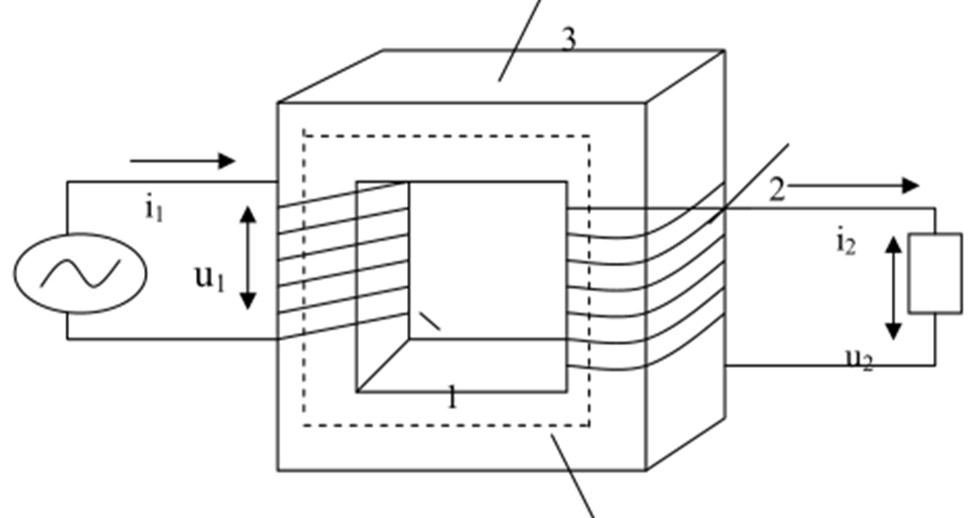
\includegraphics[width=0.4\linewidth]{figs/VN12-Y24-PH-SYL-024P-2}
	\end{center}
	\choiceTF[t]
	{Máy biến áp trên là máy hạ áp}
	{\True Điện áp ở cuộn thứ cấp là $\SI{1350}{\volt}$}
	{\True Công suất ở cuộn sơ cấp là $\SI{2700}{\watt}$}
	{\True Cường độ dòng điện ở cuộn thứ cấp là $\SI{2}{\ampere}$}
	\loigiai{
		\begin{itemchoice}
			\itemch Sai. Vì số vòng dây trên cuộn thứ cấp nhiều hơn trên cuộn sơ cấp nên là máy tăng áp.
			\itemch Đúng. $U_2=\dfrac{N_2}{N_1}U_1=\SI{1350}{\volt}$.
			\itemch Đúng. Công suất ở cuộn sơ cấp là $\calP_1=U_1I_1=\SI{2700}{\watt}$.
			\itemch Đúng. $I_2=\dfrac{\calP_2}{U_2}=\SI{2}{\ampere}$.
		\end{itemchoice}	
	}
\end{ex}
% ===================================================================
\begin{ex}
	Khi truyền tải điện năng đi xa, cần giảm công suất hao phí trên đường dây tải điện.
	\choiceTF[t]
	{Dùng dây dẫn có tiết diện nhỏ}
	{\True Tăng điện áp ở nơi nhà máy điện}
	{\True Dùng dây dẫn có điện trở suất nhỏ}
	{Giảm điện áp ở nơi sử dụng điện}
	\loigiai{
		\begin{itemchoice}
			\itemch Sai. Dùng dây dẫn có tiết diện nhỏ $\rightarrow$ điện trở lớn $\rightarrow$ toả nhiệt nhiều, đồng thời độ bền của dây kém.
			\itemch Đúng. Tăng điện áp ở nơi nhà máy điện.
			\itemch Đúng. Dùng dây dẫn có điện trở suất nhỏ $\rightarrow$ điện trở nhỏ $\rightarrow$ toả nhiệt ít.
			\itemch Sai. Lưới điện quốc gia sử dụng điện $\SI{220}{\volt}$.
		\end{itemchoice}	
	}
\end{ex}


\Closesolutionfile{ans}
\subsubsection{Tự luận}
\setcounter{ex}{0}
\Opensolutionfile{ans}[ans/VN12-Y24-PH-SYL-023P-TL]
% ======================================================================
\begin{ex}
	\immini{Máy biến áp là một thiết bị hoạt động theo nguyên lí cảm ứng điện từ nhằm thay đổi điện áp xoay chiều nhưng vẫn giữ nguyên tần số. Máy biến áp đóng vai trò rất quan trọng trong hệ thống truyền tải và phân phối điện năng. Cụ thể, để tối ưu hiệu suất của quá trình truyền tải điện năng đi xa và giảm thiểu hao phí trong quá trình này, việc sử dụng dòng điện xoay chiều với điện áp cao là cần thiết. Trước khi được truyền đi, điện áp cần được tăng lên thông qua máy tăng áp. Khi đến nơi tiêu thụ như khu công nghiệp hoặc khu dân cư, điện áp được hạ xuống thông qua máy hạ áp để phù hợp với nhu cầu sử dụng.}
	{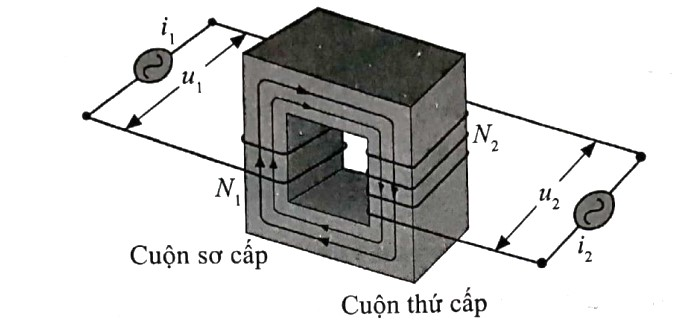
\includegraphics[scale=0.5]{figs/VN12-Y24-PH-SYL-024P-4}}
	Cấu tạo máy biến áp gồm hai bộ phận chính hình bên: lõi thép và dây quấn. Lõi thép được chế tạo bởi vật liệu dẫn từ tốt, gồm nhiều lá thép ghép cách điện với nhau. Dây quấn thường làm bằng đồng hoặc nhôm, bên ngoài có bọc cách điện.\\
	Nối cuộn dây sơ cấp của máy biến áp vào một điện áp xoay chiều $u_1=U_1 \cos \left(\omega t+\varphi_{u_1}\right)$ thì trong cuộn sơ cấp sẽ xuất hiện dòng điện sơ cấp $i_1=I_1 \cos \left(\omega t+\varphi_{i_1}\right)$ và sinh ra từ thông $\Phi(t)=\Phi_0 \cos (\omega t+\varphi)$, từ thông này xuyên qua đồng thời cả hai dây quấn sơ cấp $N_1$ và thứ cấp $N_2$. Theo định luật Faraday, chứng minh rằng, suất điện động xoay chiều xuất hiện trong dây quấn thứ cấp có cùng tần số với điện áp xoay chiều đặt vào hai đầu cuộn dây sơ cấp.
	\loigiai{
		Từ thông qua dây quấn thứ cấp là: $\Phi_2(t)=N_2 \Phi_0 \cos (\omega t+\varphi)$. Trong cuộn thứ cấp xuất hiện suất điện động là:
		$$
		e_2=-\dfrac{d \Phi_2}{dt}=N_2 \Phi_0 \omega \sin (\omega t+\varphi)
		$$
		Vậy suất điện động xoay chiều xuất hiện trong dây quấn thứ cấp có cùng tần số với điện áp xoay chiều đặt vào hai đầu cuộn dây sơ cấp.
	}
\end{ex}
% ======================================================================
\begin{ex}
	Một máy biến áp lý tưởng có 6000 vòng dây ở cuộn sơ cấp. Nó được sử dụng để chuyển đổi điện áp $\SI{230}{\volt}$ thành $\SI{9.0}{\volt}$. Tính số vòng dây của cuộn thứ cấp.	
	\loigiai{
		$\dfrac{U_2}{U_1}=\dfrac{N_2}{N_1}\Rightarrow N_2=\SI{235}{\text{vòng}}	.$
	}
\end{ex}
% ======================================================================
\begin{ex}
	Nếu đặt điện áp xoay chiều có giá trị hiệu dụng $\SI{100}{\volt}$ vào hai đầu cuộn 1 của một máy biến áp thì đo được điện áp hai đầu cuộn 2 là $\SI{50}{\volt}$. Nếu đặt điện áp có giá trị hiệu dụng $\SI{200}{\volt}$ vào hai đầu cuộn 2 thì điện áp hai đầu cuộn 1 là bao nhiêu?
	\loigiai{
		Ban đầu: $\dfrac{U_1}{U_2}=\dfrac{N_1}{N_1}=2$.\\
		Khi đặt điện áp có giá trị hiệu dụng $U'_1=\SI{200}{\volt}$ vào hai đầu cuộn 2 thì:
		$$\dfrac{U'_2}{U'_1}=\dfrac{N_1}{N_2}=2\Rightarrow U'_2=\SI{400}{\volt}.$$	
	}
\end{ex}





% ======================================================================
\begin{ex}
	\immini{	Ở các nhà máy phát điện, máy tăng áp thường được sử dụng để nâng điện áp từ mức trung thế (từ $\SI{10}{\kilo\volt}$ đến $\SI{50}{\kilo\volt}$) lên mức cao thế (từ $\SI{110}{\kilo\volt}$ đến $\SI{500}{\kilo\volt}$) trước khi truyền tải qua đường dây điện cao thế (hình bên).\\
	Một nhà máy phát điện cung cấp điện năng với công suất $\calP_0=\SI{20}{\mega\watt}$ cho một thành phố cách nhà máy $\SI{24}{\kilo\meter}$. Trước khi truyền tải, điện áp được sản xuất từ nhà máy điện có giá trị hiệu dụng khoảng $\SI{22}{\kilo\volt}$. Đường dây tải điện làm bằng đồng có điện trở suất $\SI{1.69E-8}{\ohm\cdot\meter}$ với tiết diện $\SI{0.65}{\centi\meter^2}$. 
	}
{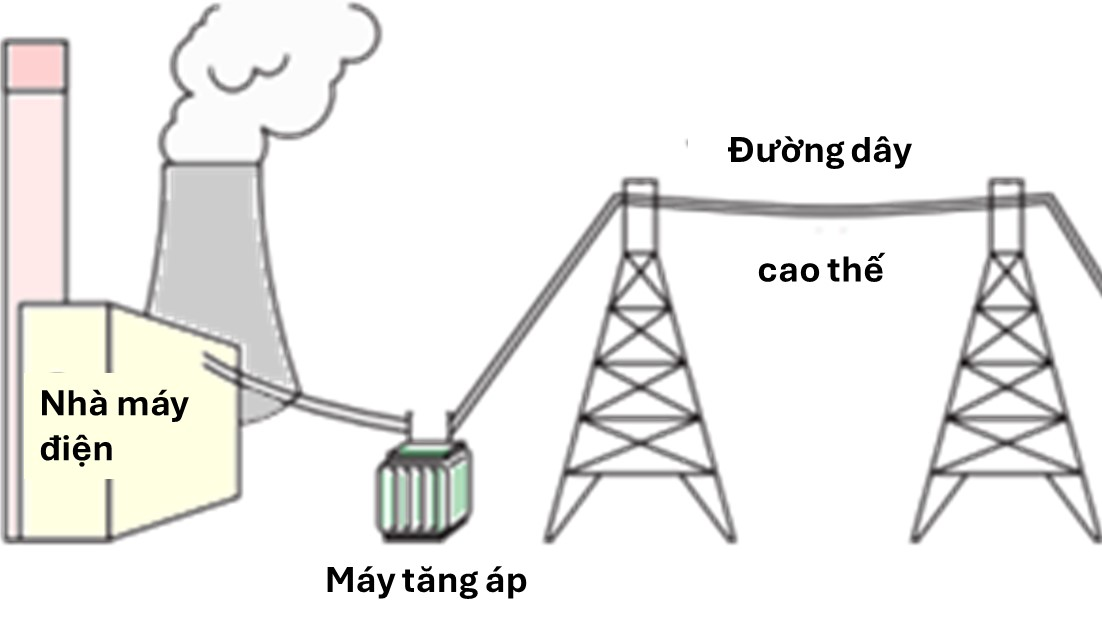
\includegraphics[scale=0.5]{figs/VN12-Y24-PH-SYL-024P-5}}
Xem các hao phí năng lượng chỉ xảy ra trên điện trở đường dây tải điện. Hãy xác định chi phí phải chi trả do hao phí năng lượng xuất hiện trên dây trong một ngày (24 giờ) ở hai trường hợp sau và nhận xét.
		\begin{enumerate}[label=\alph*)]
		\item Điện áp từ nhà máy phát điện chưa được tăng qua máy biến áp và được truyền tải đi với điện áp là $\SI{22}{\kilo\volt}$.
		\item  Điện áp từ nhà máy phát điện qua một máy tăng áp để nâng điện áp lên $\SI{220}{\kilo\volt}$ trước khi truyền tải.
	\end{enumerate}
	Lấy chi phí truyền tải trên đường dây đến thành phố đối với cả hai mức điện áp này là khoảng $\SI{145}{\text{đồng}/\kilo\watt\hour}$.
	\loigiai{
		Điện trở của đường dây tải điện là:
		$$R=\dfrac{\rho \ell}{S}=\dfrac{1,69 \cdot 10^{-8} \cdot 24 \cdot 10^3}{0,65 \cdot 10^{-4}}=\SI{6.24}{\ohm}.$$
		\begin{enumerate}[label=\alph*)]
			\item Cường độ dòng điện hiệu dụng là:
			$$
			I=\frac{\calP_0}{U}=\frac{20 \cdot 10^6}{22 \cdot 10^3} \approx \SI{909.09}{\ampere}.
			$$
			Công suất toả nhiệt trên dây dẫn là:
			$$
			\calP_R=I^2 R=909,09^2 \cdot 6,24 \approx \SI{5157.01}{\kilo\watt}.
			$$
			Năng lượng nhiệt toả ra trên dây dẫn truyền tải điện trong một ngày (24 giờ) là:
			$$
			Q=\calP_R t=5157,01\cdot24= \SI{123768.24}{\kilo\watt\hour}.
			$$
			Giá thành cần phải bỏ ra do hao phí năng lượng nhiệt xuất hiện trên dây truyền tải trong một ngày là: $123768,24\cdot145 \approx 17946395$ đồng.
			\item Sau khi tăng áp, cường độ dòng điện hiệu dụng là:
			$$
			I^{\prime}=\dfrac{\calP_0}{U^{\prime}}=\frac{20\cdot10^6}{220\cdot10^3} \approx \SI{90.91}{\ampere}.
			$$
			Công suất toả nhiệt trên dây dẫn là:
			$$
			\calP_R^{\prime}=I^{\prime 2} R=90,91^2\cdot6,24 \approx \SI{51.57}{\kilo\watt}.
			$$
			Năng lượng nhiệt toả ra trên dây dẫn truyền tải điện trong một ngày (24 giờ) là:
			$$
			Q^{\prime}=\calP_R^{\prime} t=51,57\cdot24= \SI{1237.68}{\kilo\watt\hour}.
			$$
			Giá thành cần phải bỏ ra do hao phí năng lượng nhiệt xuất hiện trên dây truyền tải trong một ngày là:
			$$
			1237,68\cdot145\approx \SI{179464}{\text{đồng}}.
			$$
			
		\end{enumerate}
	}
\end{ex}
% =============================================================
\begin{ex}
	Đặt vào hai đầu cuộn sơ cấp của máy biến áp lí tưởng (bỏ qua hao phí) một điện áp xoay chiều có giá trị hiệu dụng không đổi thì điện áp hiệu dụng giữa hai đầu cuộn thứ cấp để hở là $\SI{100}{\volt}$. Ở cuộn thứ cấp, nếu giảm bớt $n$ vòng dây thì điện áp hiệu dụng giữa hai đầu để hở của nó là $U$, nếu tăng thêm $n$ vòng dây thì điện áp đó là $2U$. Nếu tăng thêm $1,5n$ vòng dây ở cuộn thứ cấp thì điện áp hiệu dụng giữa hai đầu để hở của cuộn này bằng bao nhiêu volt?
	\loigiai{
		Ta có: $\dfrac{U_1}{U_2}=\dfrac{N_1}{N_2}$
		\begin{equation}
			\label{eq:6}\\
			\Rightarrow U_2=\dfrac{N_2U_1}{N_1}=\SI{100}{\volt}	
		\end{equation}
		\begin{equation}
			\label{eq:7}\\
			\dfrac{N_1}{N_2-n}=\dfrac{U_1}{U}
		\end{equation}
		\begin{equation}
			\label{eq:8}\\
			\dfrac{N_1}{N_2+n}=\dfrac{U_1}{2U}
		\end{equation}
		Từ \eqref{eq:7} và \eqref{eq:8}
		\begin{equation}
			\label{eq:9}\\
			\Rightarrow N_2=3n
		\end{equation}
		\begin{equation}
			\label{eq:10}\\
			\dfrac{N_1}{N_2+1,5n}=\dfrac{U_1}{U_3}\Rightarrow U_3=\dfrac{U_1}{N_1}\left(N_2+1,5n\right)
		\end{equation}
		Từ \eqref{eq:6}, \eqref{eq:9}, \eqref{eq:10} $\Rightarrow U_3=\SI{150}{\volt}$.
	}
\end{ex}
\Closesolutionfile{ans}